\documentclass[review]{elsarticle}

\usepackage{pythonhighlight}
%\journal{Journal of \LaTeX\ Templates}

%%%%%%%%%%%%%%%%%%%%%%%
%% Elsevier bibliography styles
%%%%%%%%%%%%%%%%%%%%%%%
%% To change the style, put a % in front of the second line of the current style and
%% remove the % from the second line of the style you would like to use.
%%%%%%%%%%%%%%%%%%%%%%%

%% Numbered
%\bibliographystyle{model1-num-names}

%% Numbered without titles
%\bibliographystyle{model1a-num-names}

%% Harvard
%\bibliographystyle{model2-names.bst}\biboptions{authoryear}

%% Vancouver numbered
%\usepackage{numcompress}\bibliographystyle{model3-num-names}

% Vancouver name/year
%\usepackage{numcompress}\bibliographystyle{model4-names}\biboptions{authoryear}

%% APA style
\bibliographystyle{model5-names}\biboptions{authoryear}

%% AMA style
%\usepackage{numcompress}\bibliographystyle{model6-num-names}

%% `Elsevier LaTeX' style
%\bibliographystyle{elsarticle-num}
%%%%%%%%%%%%%%%%%%%%%%%
\newcommand{\setof}[1]{\{{#1}\}}
\newcommand{\given}{|}
\newcommand{\MCMC}{\acronym{MCMC}}
\newcommand{\MH}{\acronym{M--H}}
\newcommand{\Var}{\mathrm{Var}}
\newcommand{\data}{D}
\newcommand{\pars}{\theta}
\newcommand{\best}{{\mathrm{(best)}}}
\newcommand{\better}{{\mathrm{(better)}}}
\begin{document}

\begin{frontmatter}

\title{Population Receptive Field Estimation with Metropolis-Hastings MCMC Sampling}

%% Group authors per affiliation:
\author{Mustafa Kenan Yurtcu}
\author{Fatih Serdar Saglam}


\begin{abstract}
Markov Chain Monte Carlo (MCMC) methods for sampling probability density functions have transformed the sciences, especially in performing probabilistic inferences, or fitting models to data. Here we apply the most popular MCMC algorithm called Metropolis-Hasting (M-C) on a Computational Vision Neuroscience problem which involves estimation of Population Receptive Field (pRF) parameters from Functional Magnetic Resonance Imaging (fMRI) data. We used simulated fMRI data for validation. 
\end{abstract}

\end{frontmatter}


\section{Introduction}
The pRF estimation technique is a well-studied fMRI procedure. Typically, the estimation of parameters is performed through some optimization problem. However, inspired by \cite{Adaszewski2018}, we propose a MCMC sampler that can be used as a pRF estimator.
\subsection{MCMC Sampling}
Markov Chain Monte Carlo (MCMC) methods are methods for sampling probability distribution functions or probability density functions (pdfs). MCMC methods don’t require that you have a full analytic description of the properly normalized pdf for sampling to proceed; they only require that you be able to compute
ratios of the pdf at pairs of locations. This makes MCMC methods ideal for sampling
posterior pdfs in probabilistic inferences.

In a probabilistic inference, the posterior pdf $p(\pars\given\data)$,
or pdf for the parameters $\pars$ given the data $\data$, is
constructed from the likelihood $p(\data\given\pars)$, or pdf for the
data given the parameters, and the prior pdf $p(\pars)$ for the
parameters by what's often known as ``Bayes rule'',
\begin{eqnarray}
p(\pars\given\data) = \frac{1}{Z}\,p(\data\given\pars)\,p(\pars)
\label{eq:bayes}
\end{eqnarray}
In these contexts, the constant $Z$, sometimes written as
$p(\data)$, is known by the names ``marginal likelihood'' or
``Bayes integral'' and is usually \emph{extremely hard to calculate}. But the point is that MCMC methods will not require that you know $Z$.
That is, even though you often know the function $p(\pars\given\data)$ up to a
constant factor; you can compute ratios of the pdf at pairs of points, but not the precise value at any individual point. In addition to this normalization-insensitive property of MCMC, in its simplest forms it can be run without computing any derivatives or integrals of the function.



\subsection{fMRI response of pRF}
A population receptive field (pRF) is the region of the visual field where stimuli illicit responses from a local population of neurons. In \cite{Dumoulin2008} the authors proposed a model of neuronal population receptive field defined by a two-dimensional Gaussian function:

\begin{equation}
g(x, y) = e^{-\frac{(x-x_0)^2+(y-y_0)^2}{2\sigma^2}}
\end{equation}

Recent study by \cite{Kay2013} showed that linear spatial summation model proposed by \cite{Dumoulin2008} deviates from linearity in early visual areas (e.g., V1, V2) and grows more in the anterior extrastriate areas (e.g., LO-2, VO-2) and the data is more accurately explained when this compressive static nonlinearity is applied after linear summation.

According to the Compressive Spatial Summation (CSS) model proposed by \cite{Kay2013}, the pRF response is modeled as the element-wise (Hadamard) product of effective stimulus $s(x, y, t)$ and the Gaussian pRF model $g(x, y)$ then raised to power $n$ and multiplied with a gain factor $g$.
\begin{equation}
r(t) = g (\sum_{x, y} s(x, y, t) g(x, t))^n
\end{equation}

Next, according to a linear Hemodynamic model for the BOLD response we can model the fMRI data by a convolution with a given Hemodynamic Response Function $h(t)$,

\begin{equation}
	d(t) = r(t) * h(t)
\end{equation}

\section{Metropolis-Hastings Sampling}
The simplest algorithm for MCMC is the Metropolis-Hastings algorithm\citep{Hastings1970}. The M-H MCMC algorithm requires two inputs. The first is a handle to the function $f(\pars)$ that is the function to be sampled, such that the algorithm can evaluate $f(\pars)$ for any value of the parameters $\pars$. In data-analysis contexts, this function would be
the prior $p(\pars)$ times the likelihood $p(D | \pars)$ evaluated at the observed data $D$. The second input is a handle to a proposal pdf function $q(\pars' | \pars)$ that can deliver samples, such that the algorithm can draw a new position $\pars'$ in the parameter space given an "old" position $\pars$. It permits us to random-walk around the parameter space in a fair way.

The algorithm is the following: We have generated some set of samples, the most
recent of which is $\pars_k$. To generate the next sample $\pars_{k+1}$ do the following:
\begin{itemize}
	\item Draw a proposal $\pars'$ from the proposal pdf $q(\pars'|\pars_k)$.
	\item Draw a random number $0<r<1$ from the uniform distribution.
	\item If $f(\pars') / f(\pars_k) > r$ then $\pars_{k+1} \leftarrow \pars'$;
	otherwise $\pars_{k+1} \leftarrow \pars_k$.
\end{itemize}

That is, at each step, either a new proposed position in the parameter space gets
accepted into the list of samples or else the previous sample in the parameter space
gets repeated.

\paragraph{Importantly}—for the algorithm given above to work correctly, the proposal pdf must satisfy a "detailed-balance" condition; it must have the property that
\begin{eqnarray}
q(\pars'\given\pars) &=& q(\pars\given\pars')
\label{eq:detailed-balance}\quad
\end{eqnarray}

\section{Metropolis-Hastings Implementation}
Since we assume that the fMRI response is corrupted by additive Gaussian noise, the likelihood function becomes,

\begin{eqnarray}
	f(d(t)\given\pars) = \frac{1}{\sqrt{2\pi n_0^2}}\exp{-\frac{(d(t) - \hat{d}(t;\pars)^2}{2 n_0^2}}
\end{eqnarray}

where $n_0^2$ is the noise variance and the prediction function is given by,

\begin{eqnarray}
\hat{d}(t;\pars) = h(t)* (g (\sum_{x, y} s(x, y, t) g(x, t))^n)
\end{eqnarray}

Now assuming Gaussian distribution with zero mean for the parameters (let $g$ and $n$ be constants) we are assured that the "detailed-balance" condition is satisfied. Then we can implement the M-H algorithm with Python code as follows,
\begin{python}
	def metropolis_hastings(p, iter=1000):
		x, y, s = 0., 0., 0.
		samples = np.zeros((iter, 3))
		
		for i in range(iter):
			x_star, y_star, s_star = np.array([x, y, s]) + np.random.normal(size=3)
			if np.random.rand() < p(x_star, y_star, s_star) / p(x, y, s):
				x, y, s = x_star, y_star, s_star
			samples[i] = np.array([x, y, s])
		
		return samples
\end{python}

Since the likelihood function is Gaussian, we can find the the estimated parameter by averaging over samples and the time points,

\begin{equation}
	\hat{\theta} = \frac{1}{NK}\sum_{t=1}^{N}\sum_{k=1}^{K} \pars_k(t)
\end{equation}
\section{Simulation Result}
After a whole fMRI experiment with stimulus shown in Figure 1 is simulated, we have obtained 30x30=900 time series each corresponding to the response of a population receptive field in the visual field. After applying the estimation technique on each time series, we compared the estimation error percentages from the true values. Then we illustrated the error plots for different assumed values of the parameter $n$.
\begin{figure}[htp]
	\centering
	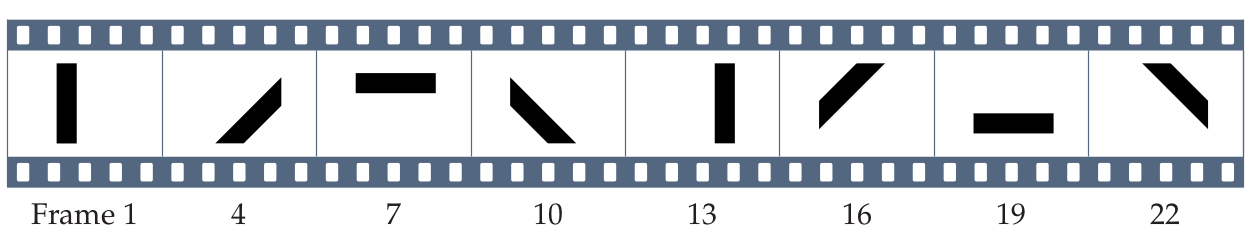
\includegraphics[width=\textwidth]{stim.png}

	\caption{Stimulus frames used for simulation}
\end{figure}

\begin{figure}[htp]
	\centering
	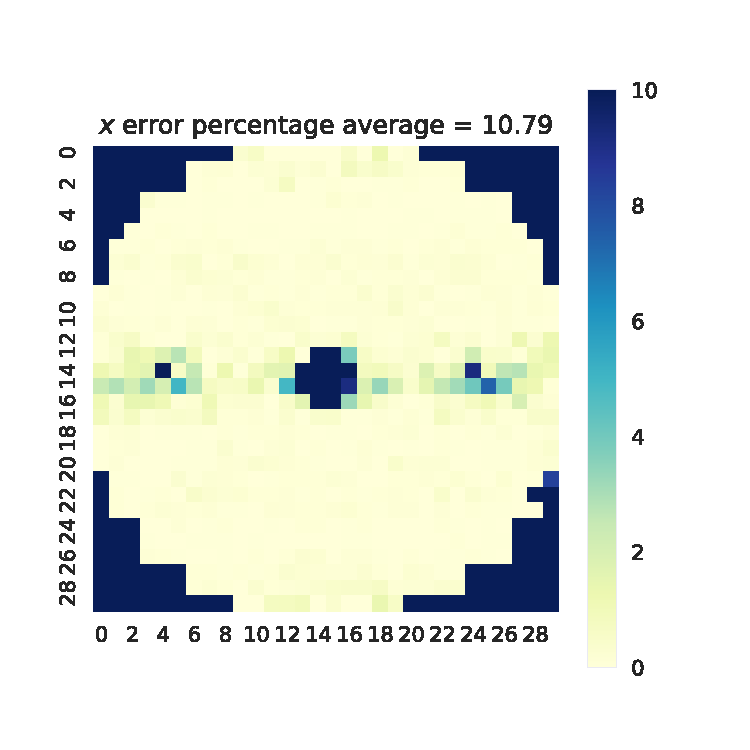
\includegraphics[width=.32\textwidth]{x_10}
	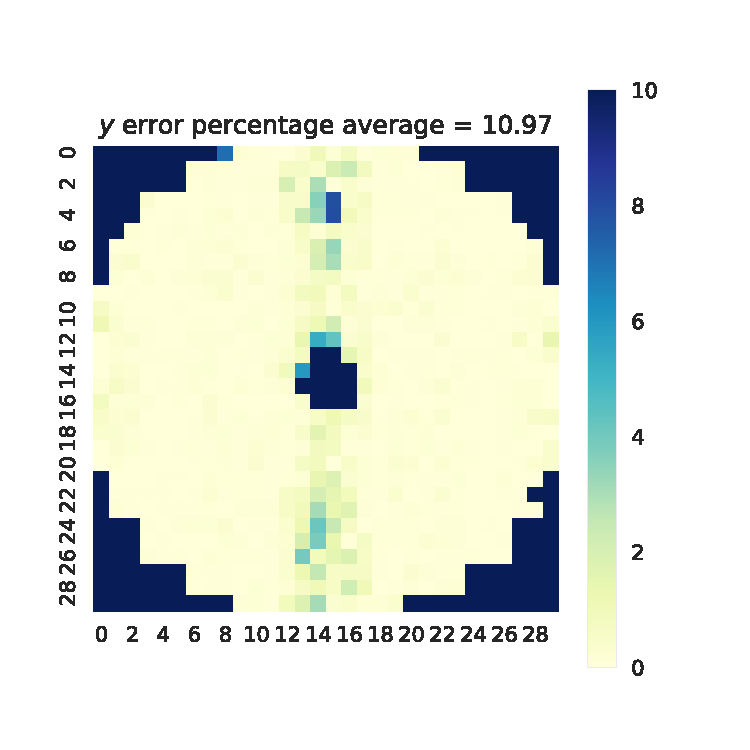
\includegraphics[width=.32\textwidth]{y_10}
	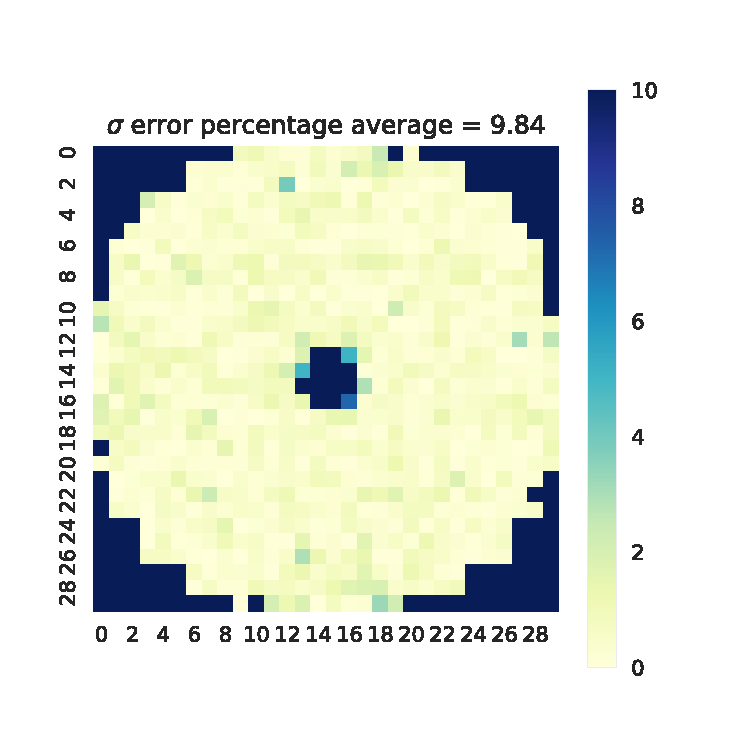
\includegraphics[width=.32\textwidth]{sigma_10}
	\vspace{-0.5cm}
	\caption{Linear model with $n=1.0$}
	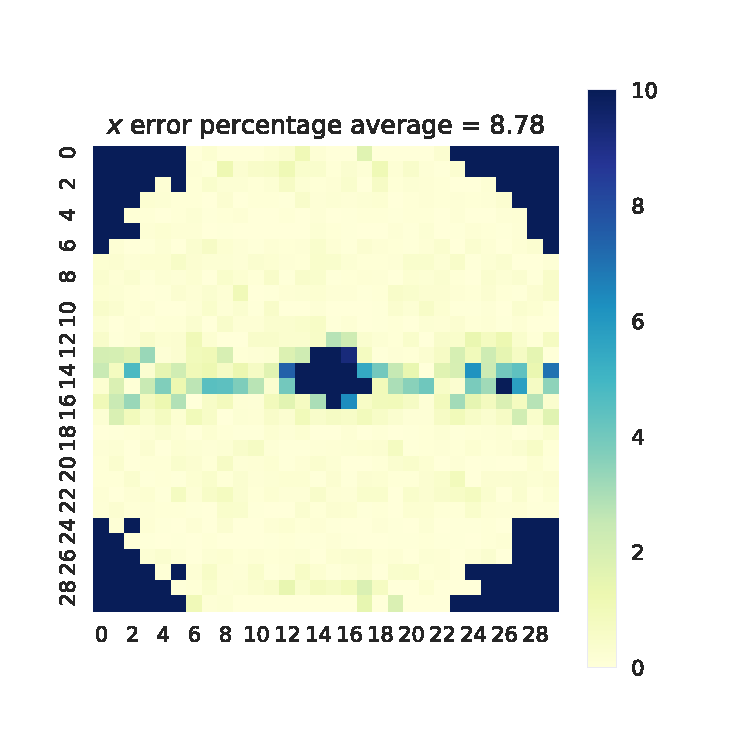
\includegraphics[width=.32\textwidth]{x_9}
	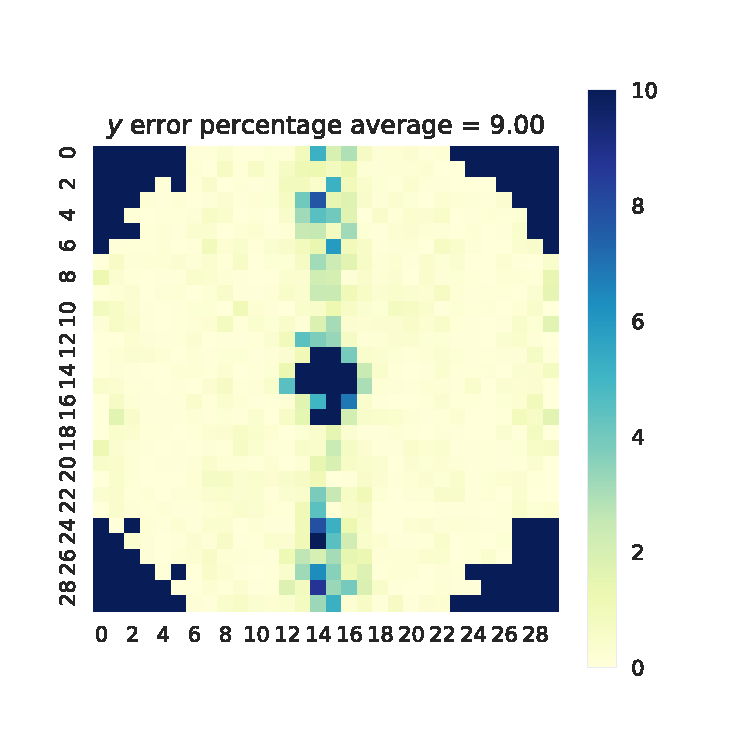
\includegraphics[width=.32\textwidth]{y_9}
	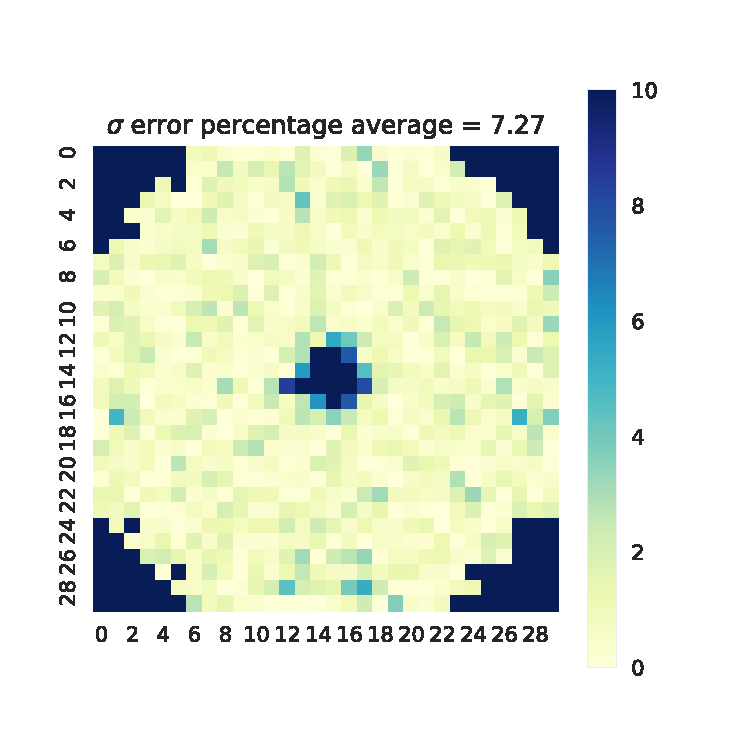
\includegraphics[width=.32\textwidth]{sigma_9}
	\vspace{-0.5cm}
	\caption{CSS model with exponent $n=0.9$}
	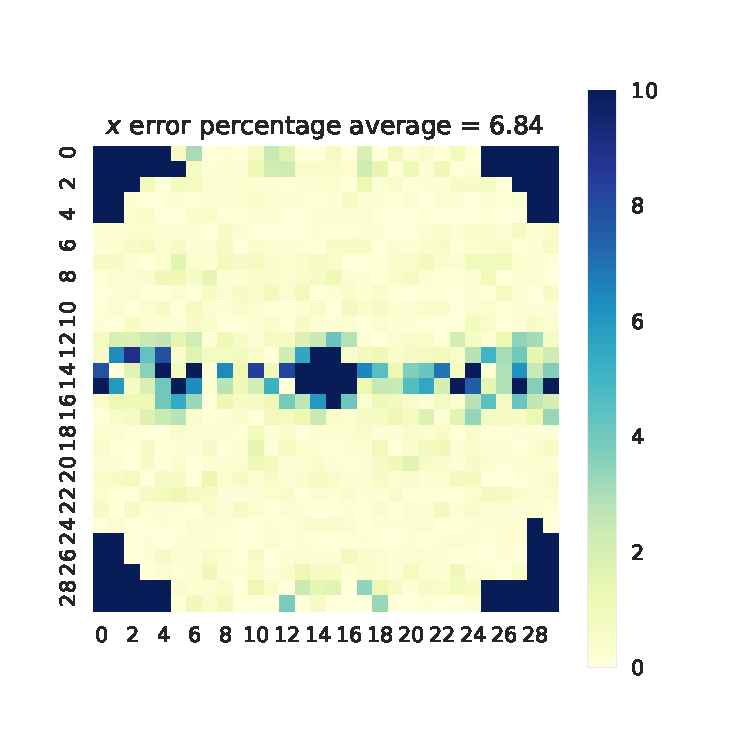
\includegraphics[width=.32\textwidth]{x_8}
	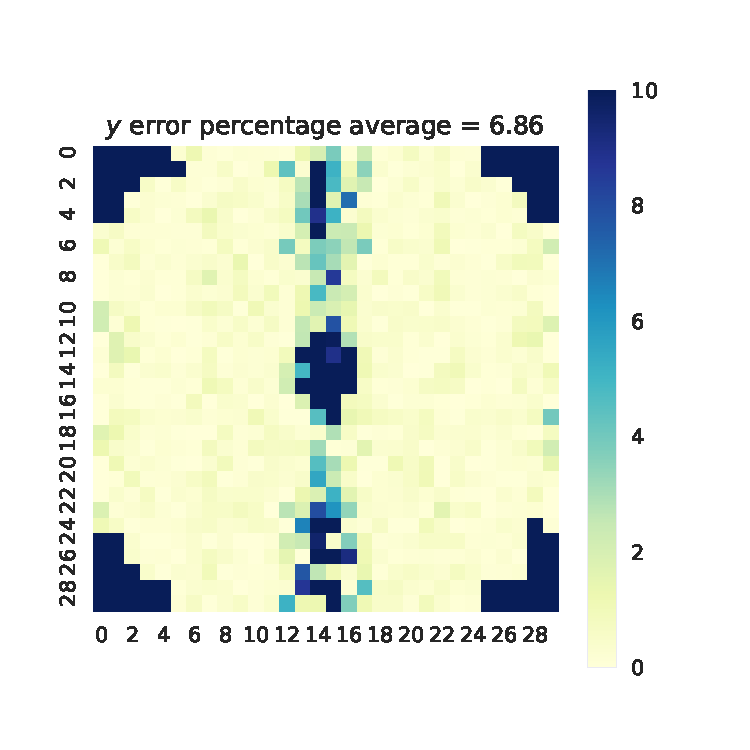
\includegraphics[width=.32\textwidth]{y_8}
	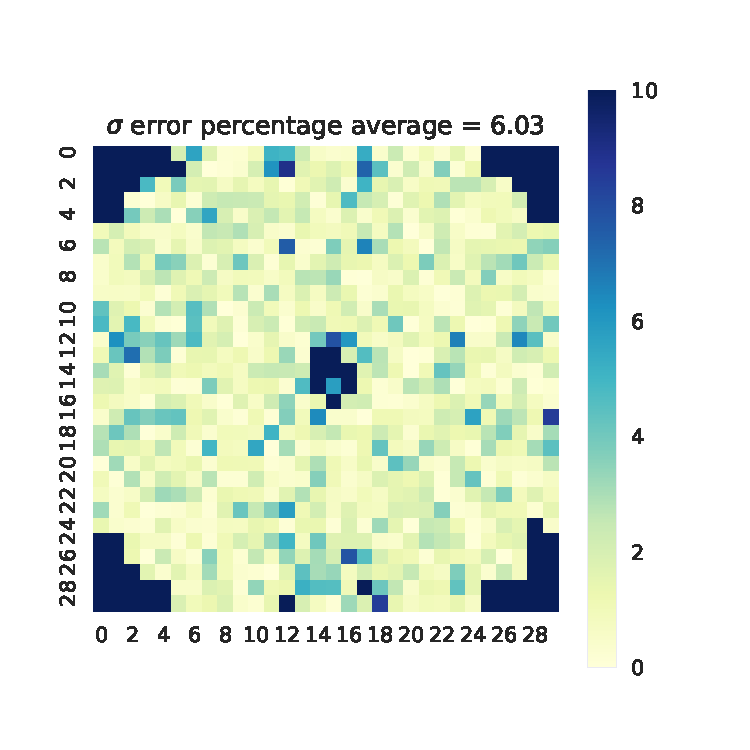
\includegraphics[width=.32\textwidth]{sigma_8}
	\vspace{-0.5cm}
	\caption{CSS model with exponent $n=0.8$}
\end{figure}
\begin{figure}[htp]
	\centering
	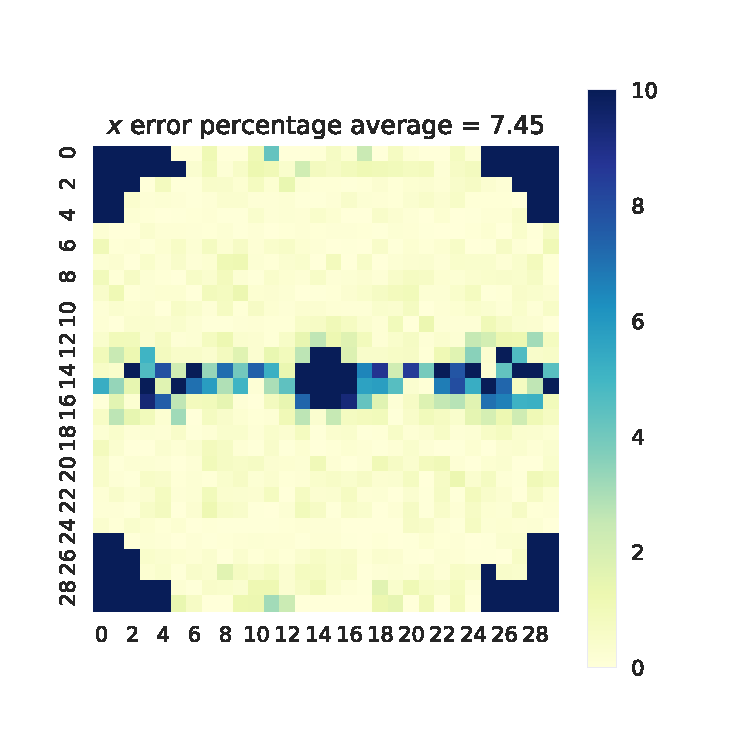
\includegraphics[width=.32\textwidth]{x_7}
	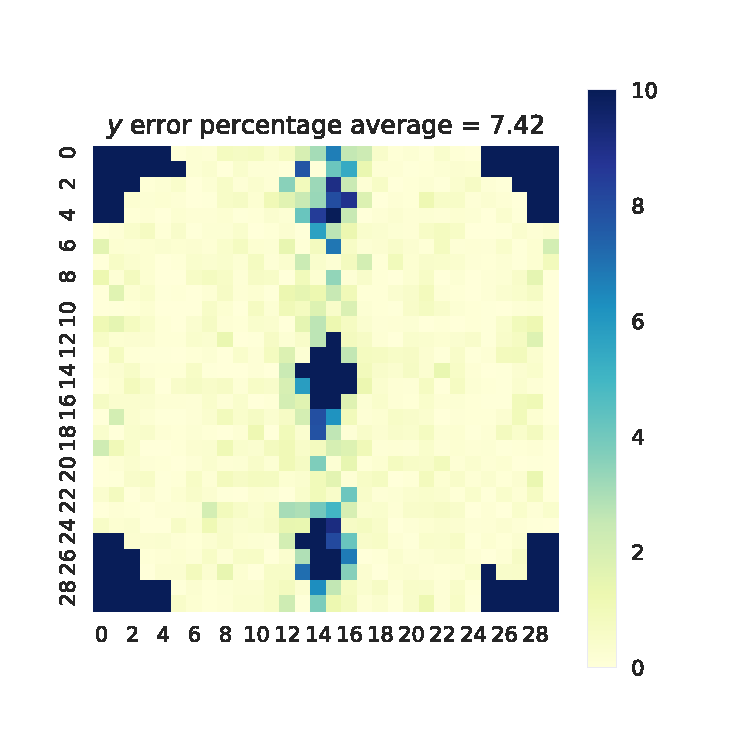
\includegraphics[width=.32\textwidth]{y_7}
	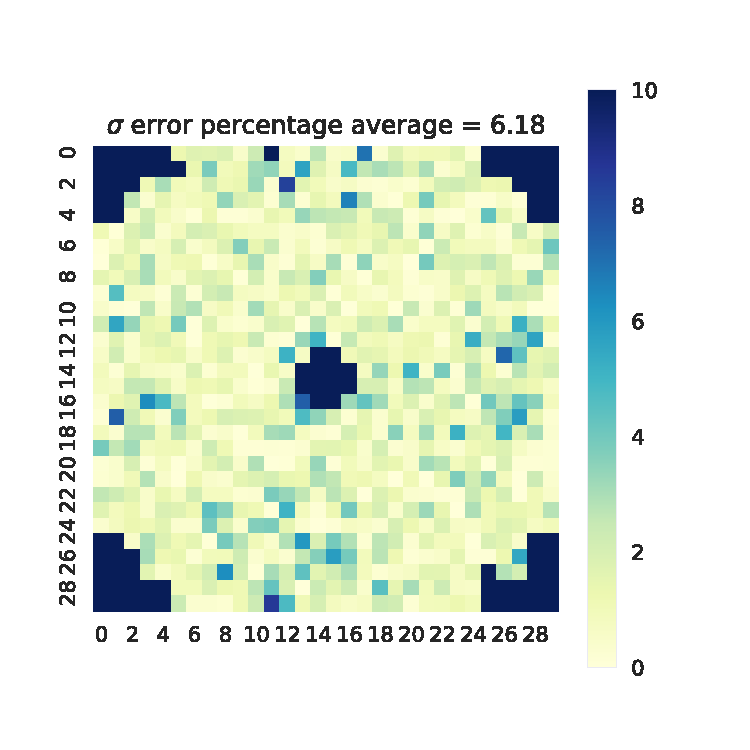
\includegraphics[width=.32\textwidth]{sigma_7}
	\vspace{-0.5cm}
	\caption{CSS model with exponent $n=0.7$}
	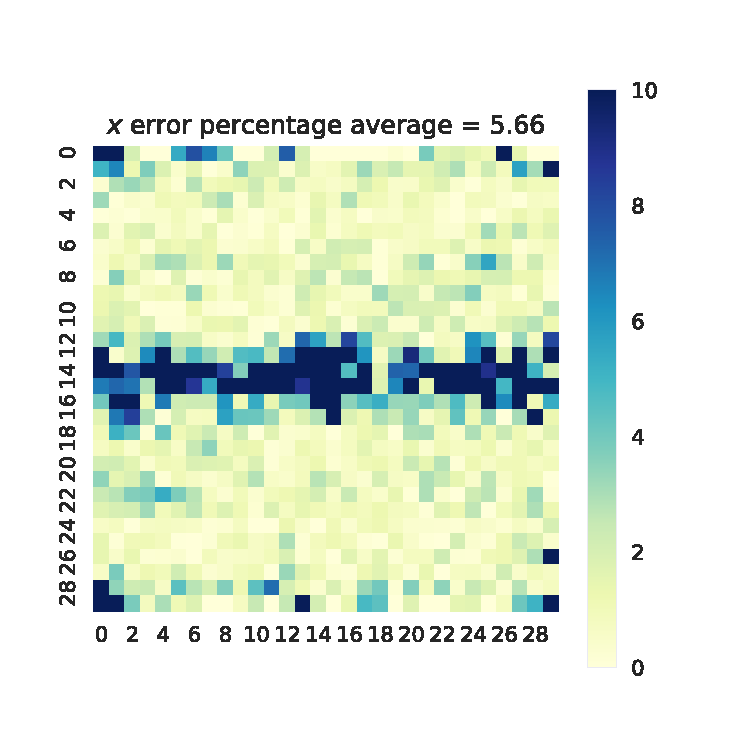
\includegraphics[width=.32\textwidth]{x_6}
	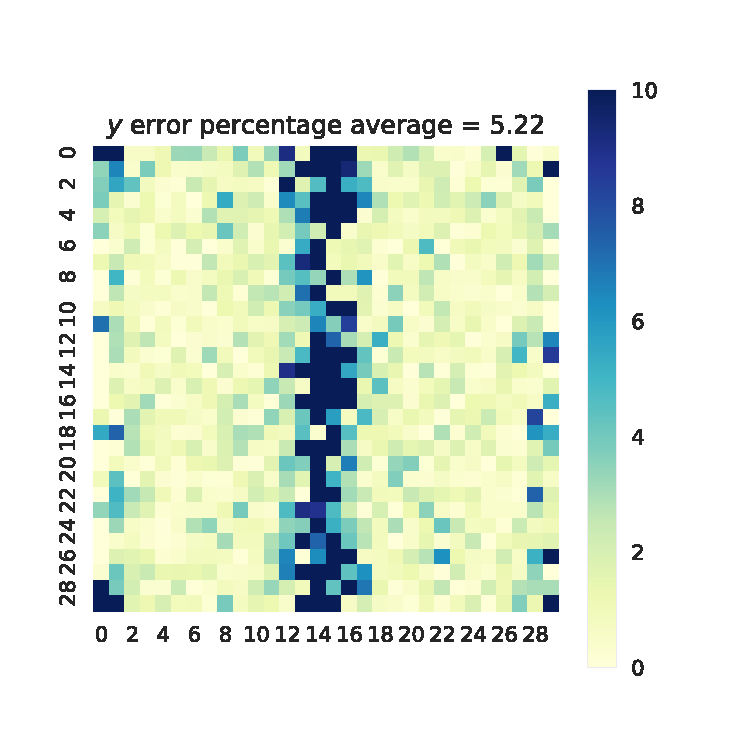
\includegraphics[width=.32\textwidth]{y_6}
	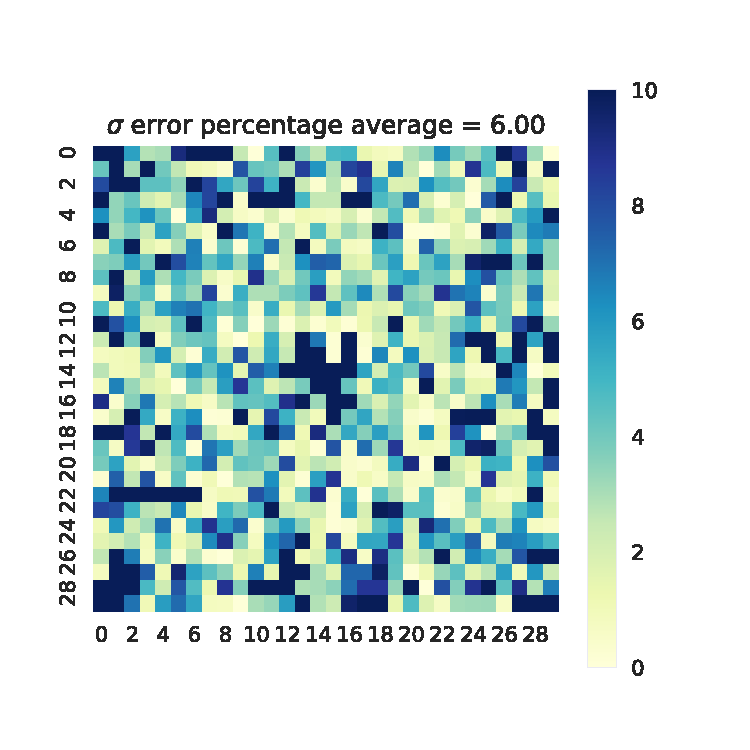
\includegraphics[width=.32\textwidth]{sigma_6}
	\vspace{-0.5cm}
	\caption{CSS model with exponent $n=0.6$}
	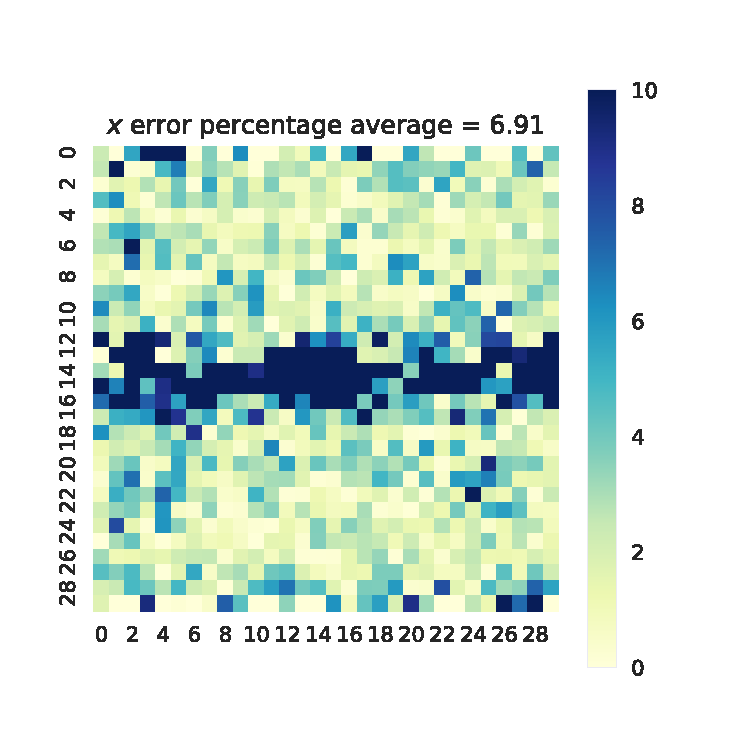
\includegraphics[width=.32\textwidth]{x_5}
	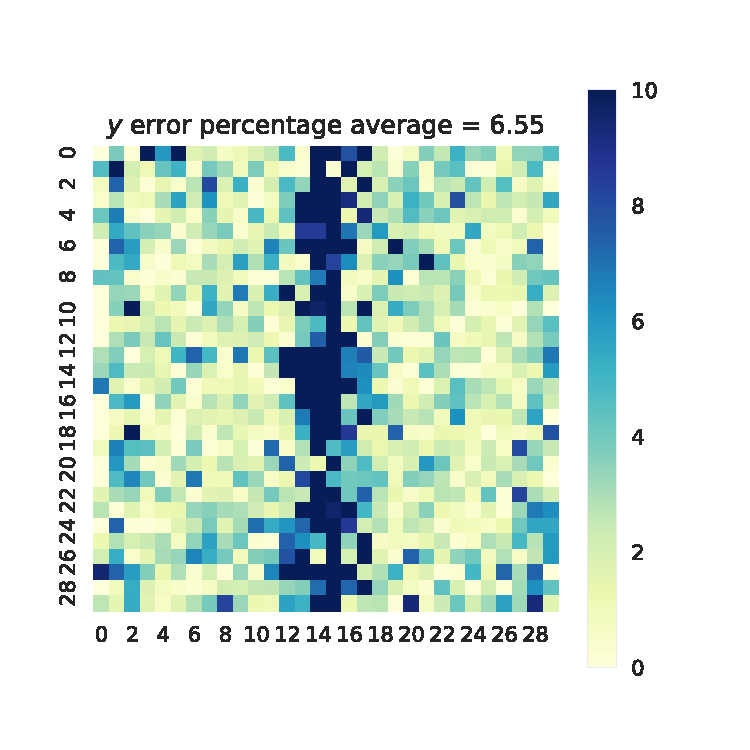
\includegraphics[width=.32\textwidth]{y_5}
	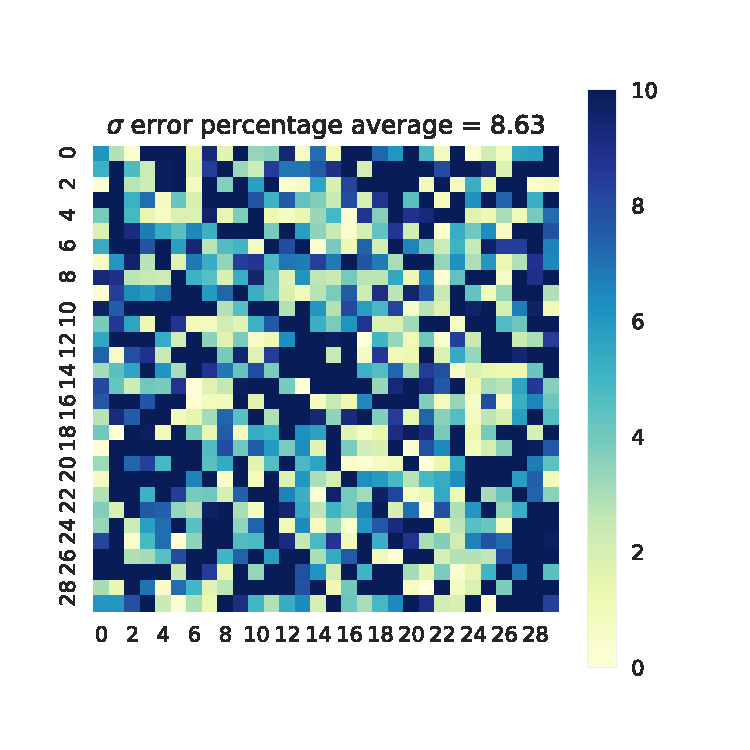
\includegraphics[width=.32\textwidth]{sigma_5}
	\vspace{-0.5cm}
	\caption{CSS model with exponent $n=0.5$}
\end{figure}

\section{Discussion and Conclusion}
In this study we have applied a straight forward MCMC sampling method to a seemingly unrelated problem in Neuroscience. The results show that this sampler can be effectively used as an estimation method for pRF parameters from fMRI data.

Furthermore, we have found interesting results in the spatial patterns of estimation errors. From Figures 2 and 7 we see that the average errors decrease when we apply static compressive nonlinearity upto $n=0.6$.

The reason for this can be seen from the error map of individual voxels. As n decreases (i.e., more spatial compressing) the receptive field away from the fixation point become easier to estimate (i.e., lower estimation error) which means they become more responsive to the stimuli.

However, with more spatial comprression the noise also gets amplified and eventually the average errors increase as shown from Figures 5 and 6. Therefore, there is a trade-off and an optimal exponent value which gives the highest average estimation power over all voxels.

Since it is shown by \cite{Kay2013} that exponent values are decreasing from unit value (i.e., increased spatial nonlinearity) for early to higher visual field areas, we can simulate these areas more realistically by using CSS pRF response model. Furthermore, our simulation results can simulate the signal-to-noise ratios of different visual areas based on these empirical exponent values.
\bibliography{mybibfile}

\end{document}